\documentclass[12pt]{article}
\usepackage[utf8]{inputenc}
\usepackage{amsmath, amssymb, amsthm, graphicx, fancyvrb, enumitem, titlesec, setspace, float, fancyvrb, minted}
\usepackage[dvipsnames]{xcolor}
\usepackage[top=1in, bottom=1in, left=1.25in, right=1.25in]{geometry}
\titleformat{\section}{\normalfont\bfseries}{}{0em}{}
\titlespacing*{\section}{0pt}{1.5ex plus .2ex minus .2ex}{0.8ex plus .1ex}


\begin{document}
\noindent Andre Winkel \hfill \today \\
\rule{\textwidth}{0.4pt} \vspace{0em}
\begin{center} \large{Lab 4} \end{center} \vspace*{0em}

\section*{Problem 1: Implementing periodic convolution}
In this problem, we will implement periodic convolution and compare it with the frequency domain implementation.
\begin{enumerate}[label=\textbf{\alph*)}, leftmargin=2.6em]

\item We start by creating and plotting one period of the two periodic signals $x[n]$ and $y[n]$:
\begin{figure}[H]
    \centering
    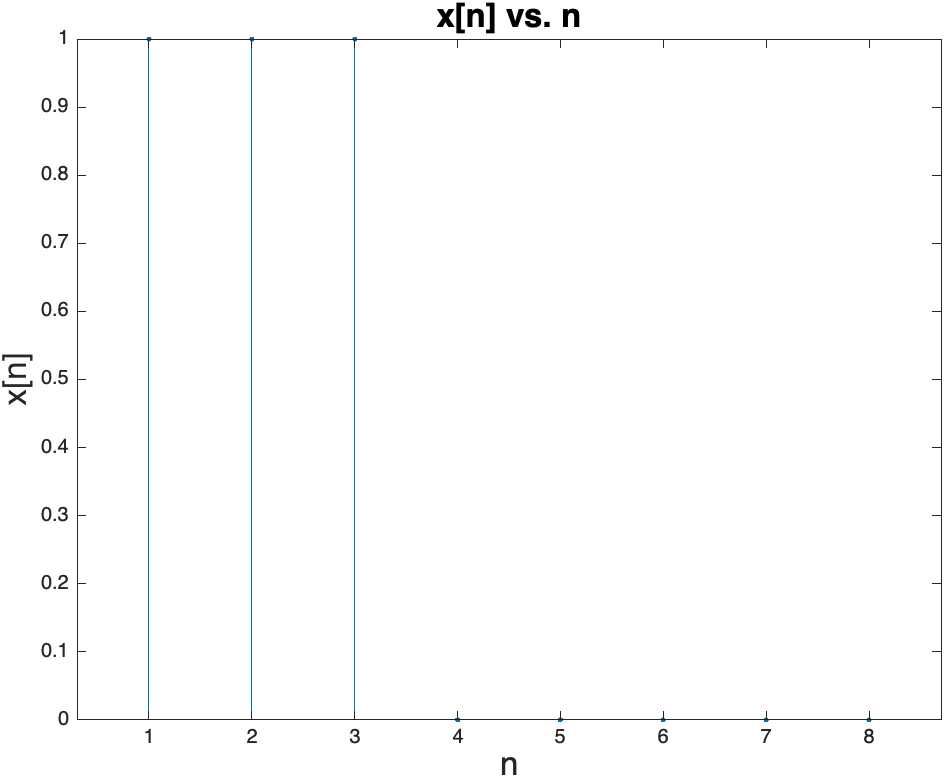
\includegraphics[width=0.35\linewidth]{1.png}
    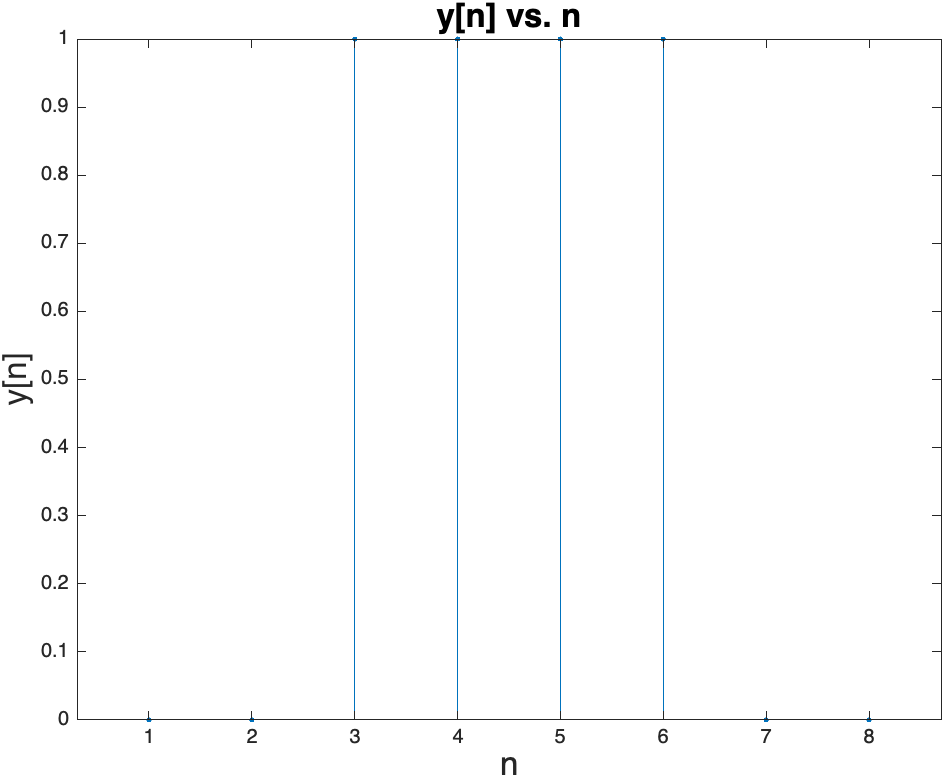
\includegraphics[width=0.35\linewidth]{2.png}
\end{figure}
\begin{minted}[frame=single, fontsize=\small, linenos, bgcolor=white]{matlab}
n = 1:8
x_arr = zeros(1,8);
y_arr = zeros(1,8);
x_arr(1:3) = 1;
y_arr(3:6) = 1;

stem(n, x_arr, '.')
title('x[n] vs. n', 'FontSize', 16)
xlabel('n', 'FontSize', 16);
ylabel('x[n]', 'FontSize', 16);

stem(n, y_arr, '.')
title('y[n] vs. n', 'FontSize', 16)
xlabel('n', 'FontSize', 16);
ylabel('y[n]', 'FontSize', 16);
\end{minted}

\item Plotting $x[n]$ for $n=-8$ to $n=15$, we observe the following:
\begin{figure}[H]
    \centering
    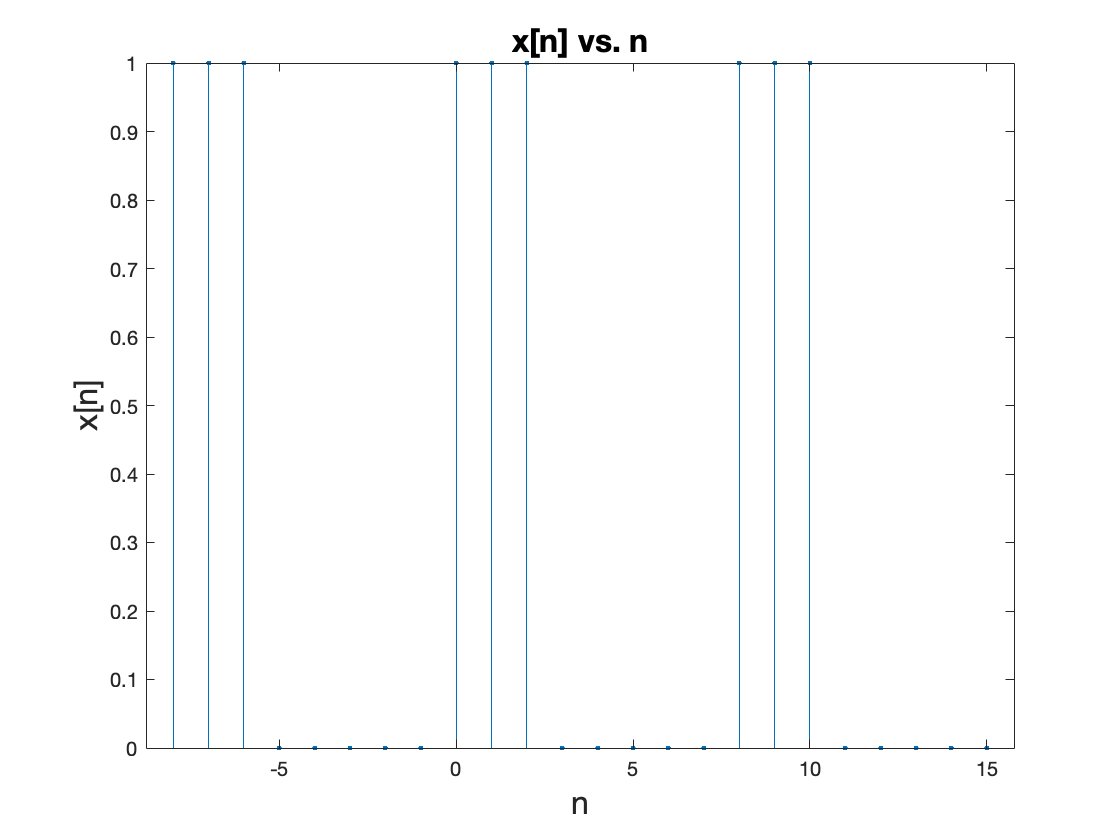
\includegraphics[width=0.5\linewidth]{3.png}
\end{figure}
\begin{minted}[frame=single, fontsize=\small, linenos, bgcolor=white]{matlab}
n = -8:15;
x_arr3 = zeros(1, length(n));
for i = 0:2
    x_arr3(8*i+1:8*(i+1))=x_arr
end

stem(n, x_arr3, '.')
title('x[n] vs. n', 'FontSize', 16)
xlabel('n', 'FontSize', 16);
ylabel('x[n]', 'FontSize', 16);
\end{minted}

\item Plotting $x[n-1]$, $x[n-4]$, and $x[n-7]$ for the same values of $n$, we obtain the following plots:
\begin{figure}[H]
    \centering
    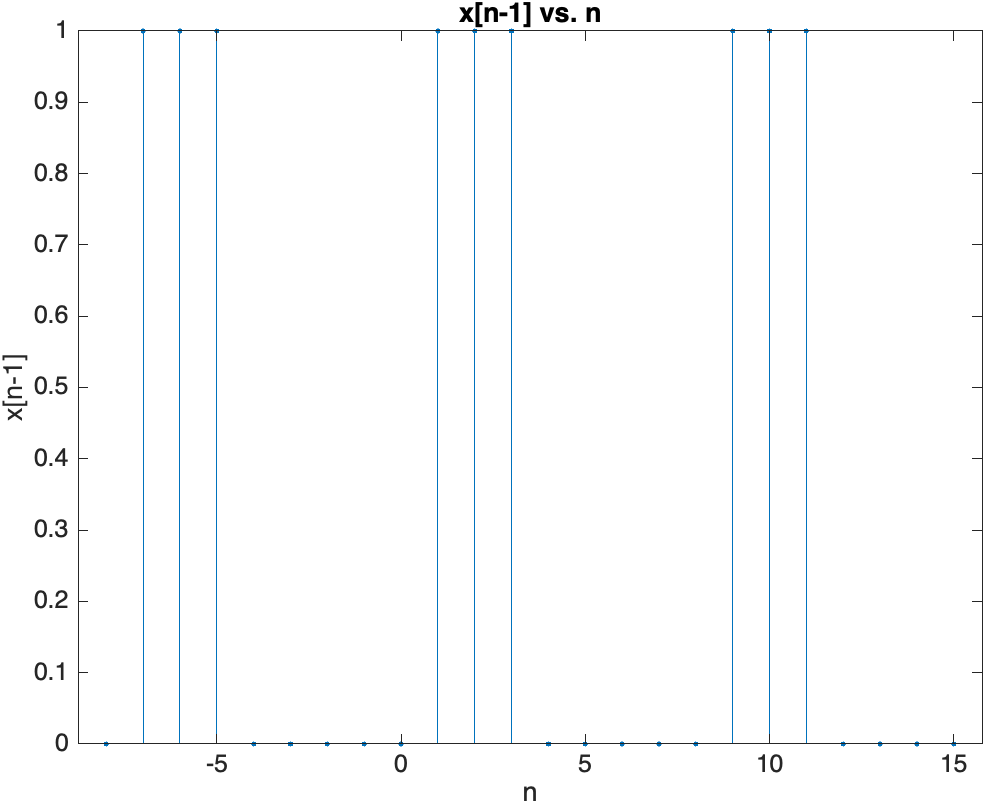
\includegraphics[width=0.32\linewidth]{4.png}
    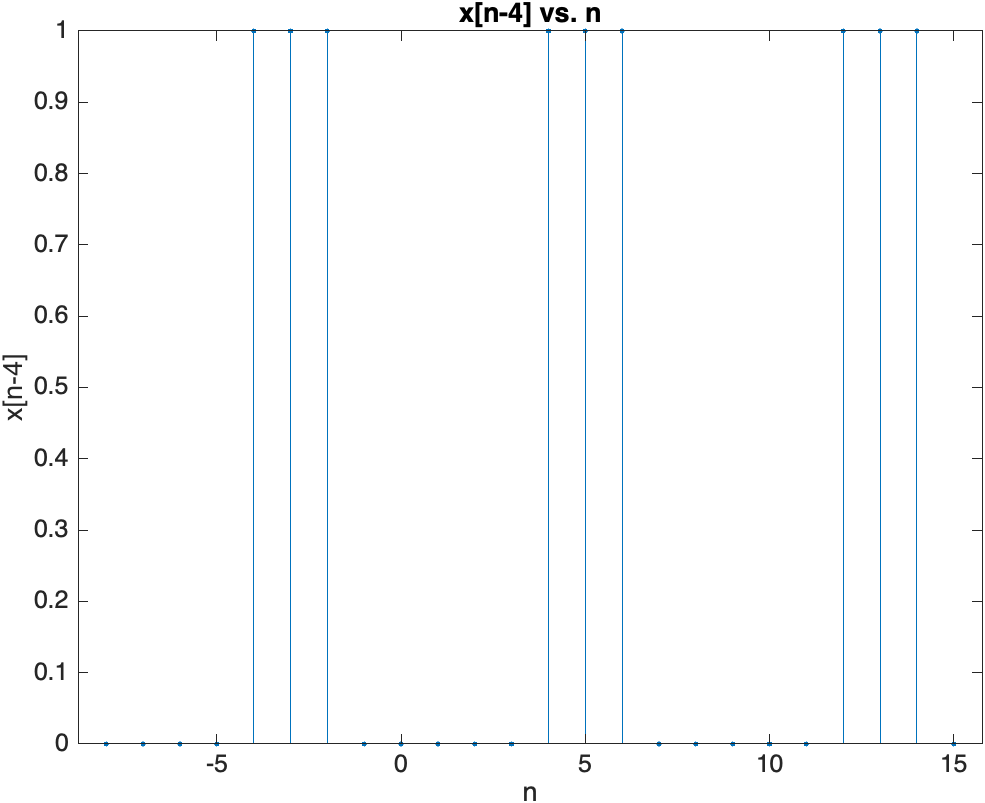
\includegraphics[width=0.32\linewidth]{5.png}
    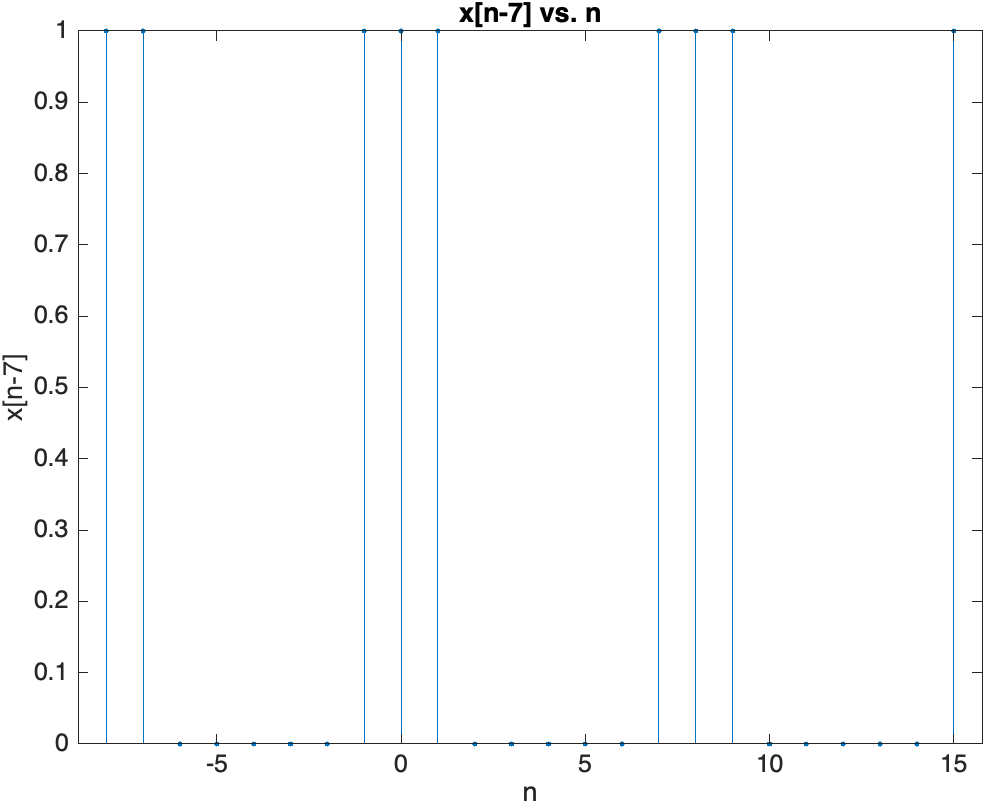
\includegraphics[width=0.32
    \linewidth]{6.png}
\end{figure}
\begin{minted}[frame=single, fontsize=\small, linenos, bgcolor=white]{matlab}
x_ext=x_arr3;
x_ext(25:48)=x_arr3;

shiftval=1;
stem(n, x_ext(9-shiftval:32-shiftval), '.');
title('x[n-1] vs. n', 'FontSize', 16);
xlabel('n', 'FontSize', 16);
ylabel('x[n-1]', 'FontSize', 16);

shiftval=4;
stem(n, x_ext(9-shiftval:32-shiftval), '.');
title('x[n-4] vs. n', 'FontSize', 16);
xlabel('n', 'FontSize', 16);
ylabel('x[n-4]', 'FontSize', 16);

shiftval=7;
stem(n, x_ext(9-shiftval:32-shiftval), '.');
title('x[n-7] vs. n', 'FontSize', 16);
xlabel('n', 'FontSize', 16);
ylabel('x[n-7]', 'FontSize', 16);
\end{minted}

\item Plotting \verb|circshift(x_arr, shift_val)| for \verb|shift_val| sequentially taking $0,1,4,7$, we can observe the following plots:
 
\begin{figure}[H]
    \centering
    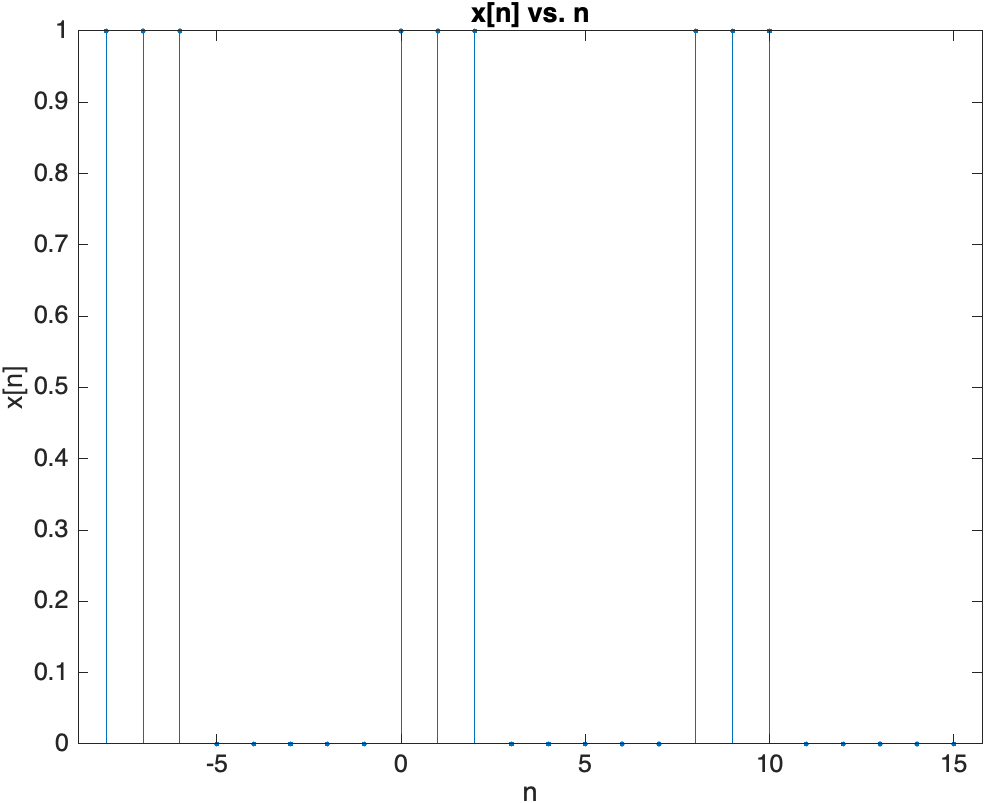
\includegraphics[width=0.49\linewidth]{circ1.png}
    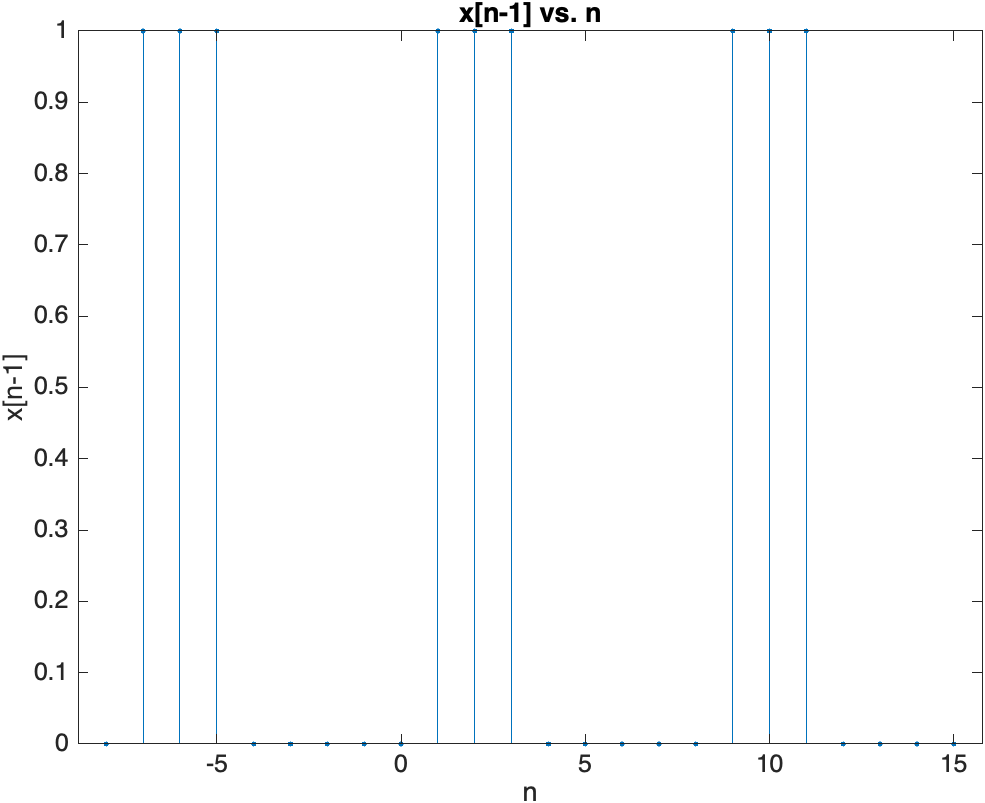
\includegraphics[width=0.49\linewidth]{circ2.png}
    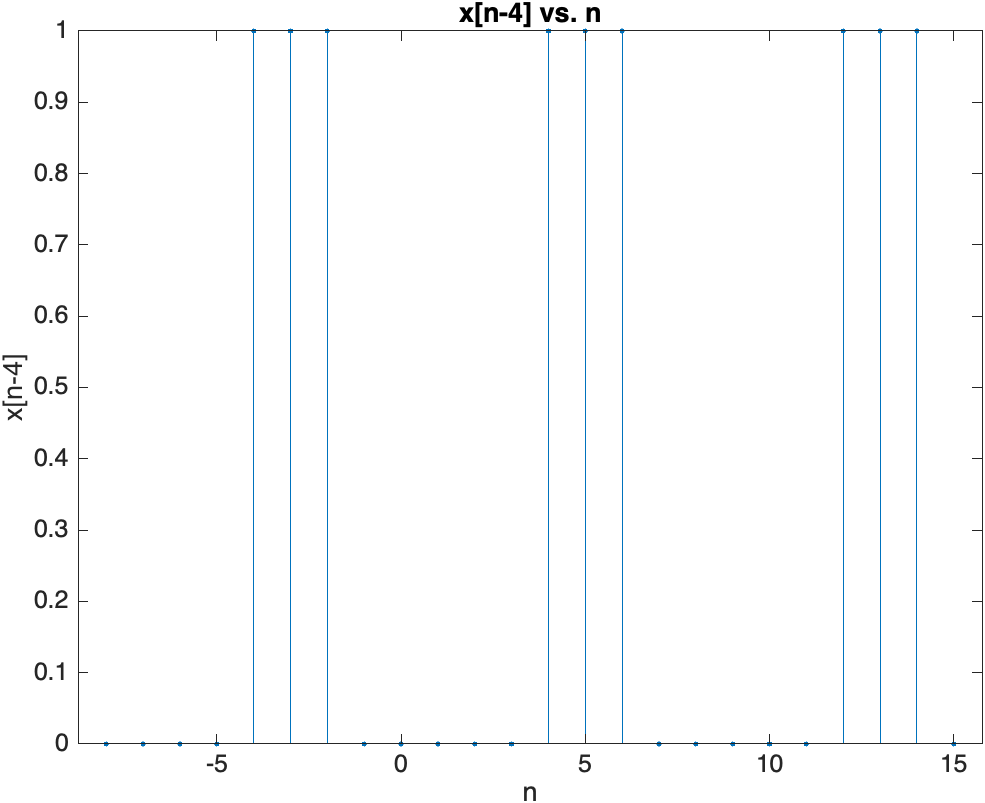
\includegraphics[width=0.49\linewidth]{circ3.png}
    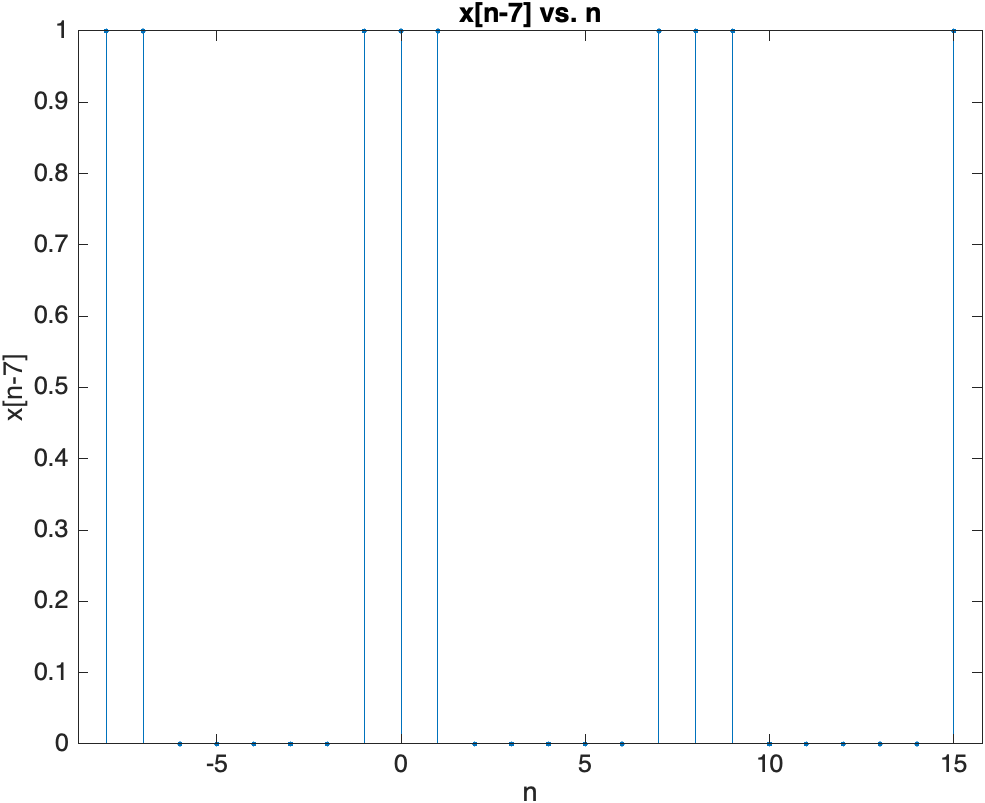
\includegraphics[width=0.49\linewidth]{circ4.png}
\end{figure}
\begin{minted}[frame=single, fontsize=\small, linenos, bgcolor=white]{matlab}
stem(n, circshift(x_arr3, 0), '.');
title('x[n] vs. n', 'FontSize', 16);
xlabel('n', 'FontSize', 16);
ylabel('x[n]', 'FontSize', 16);

stem(n, circshift(x_arr3, 1), '.');
title('x[n-1] vs. n', 'FontSize', 16);
xlabel('n', 'FontSize', 16);
ylabel('x[n-1]', 'FontSize', 16);

stem(n, circshift(x_arr3, 4), '.');
title('x[n-4] vs. n', 'FontSize', 16);
xlabel('n', 'FontSize', 16);
ylabel('x[n-4]', 'FontSize', 16);

stem(n, circshift(x_arr3, 7), '.');
title('x[n-7] vs. n', 'FontSize', 16);
xlabel('n', 'FontSize', 16);
ylabel('x[n-7]', 'FontSize', 16);
\end{minted}
We see here that the signals we obtain through our \verb|circshift(x_arr, shift_val)| implementation are exactly the same as our initial periodic time shift implementation in parts \textbf{(b)} and \textbf{(c)}.

\item In this part, we will implement periodic convolution $c[n]=x[n]\tilde{\ast}y[n]$. We will leverage Matlab's \verb|circshift| command in order to convolve with period signals, considering periodic convolution is between two signals of infinite length with values repeating every $N$ units, where $N$ is the period of the signal. We observe the periodic convolution $c[n]$ below:
\begin{figure}[H]
    \centering
    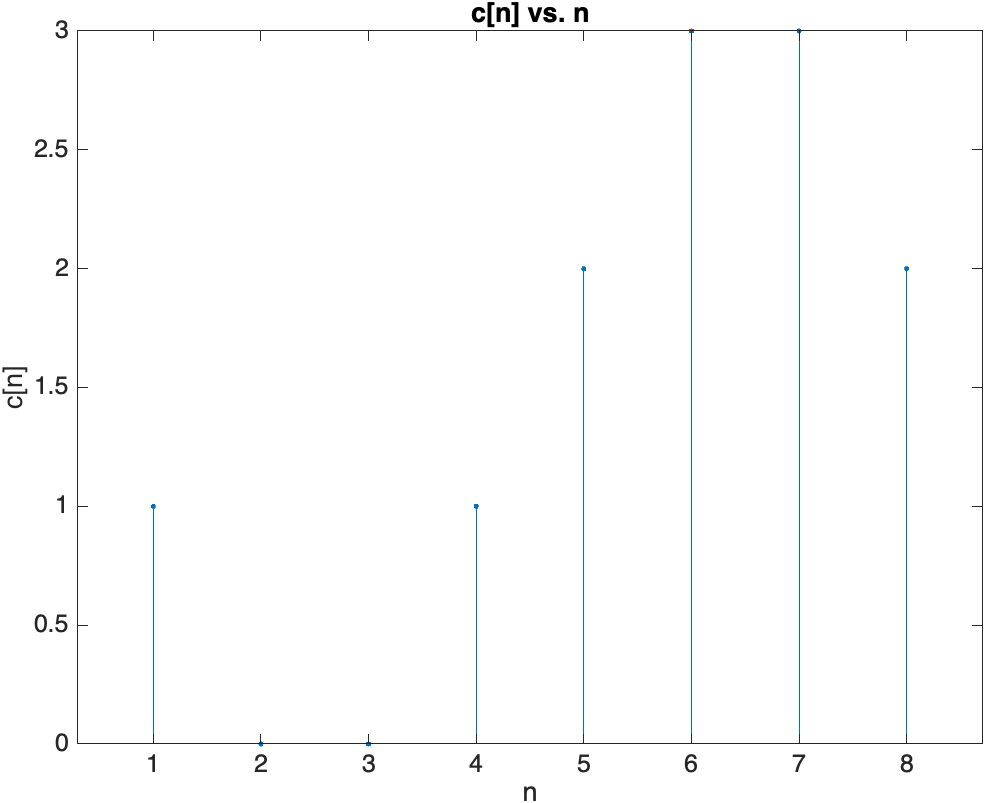
\includegraphics[width=0.5\linewidth]{conv1.png}
\end{figure}
\begin{minted}[frame=single, fontsize=\small, linenos, bgcolor=white]{matlab}
N = 8;
c_arr = zeros(1, N);
% Remember that convolution has to happen over any one period. 
% 1:N is convenient
for idx = 1:N
    % First flip
    y_flipped = y_arr(N:-1:1);

    % Then advance using circshift
    y_shifted = circshift(y_flipped, idx-1);
    c_arr(idx) = sum(x_arr.*y_shifted);
end

stem(1:N, c_arr, '.')
title('c[n] vs. n', 'FontSize', 16);
xlabel('n', 'FontSize', 16);
ylabel('c[n]', 'FontSize', 16);
\end{minted}

\item We can compute the discrete time Fourier transform coefficients, $a_k$ of $x[n]$ and $b_k$ of $y[n]$, using the Matlab command \verb|fft|. It is important to note the Matlab equations for DTFS,
\begin{equation}
    a_k^{\text{Matlab}}=\sum_{n=1}^N x[n]e^{-j\omega_0(k+1)(n-1)}
\end{equation}
and
\begin{equation}
    x[n]=\frac{1}{N}\sum_{k=1}^N a_k^{\text{Matlab}}x[n]e^{-j\omega_0(k-1)(n+1)},
\end{equation}
are slightly different than our typical application. Using \verb|fft|, we can obtain said coefficients. We can then compute $c_k=a_kb_k$, and the signal $z[n]$ that has $c_k$ as its coefficients through the \verb|ifft| command. 

\item We can observe the plot of $z[n]$ below:
\begin{figure} [H]
    \centering
    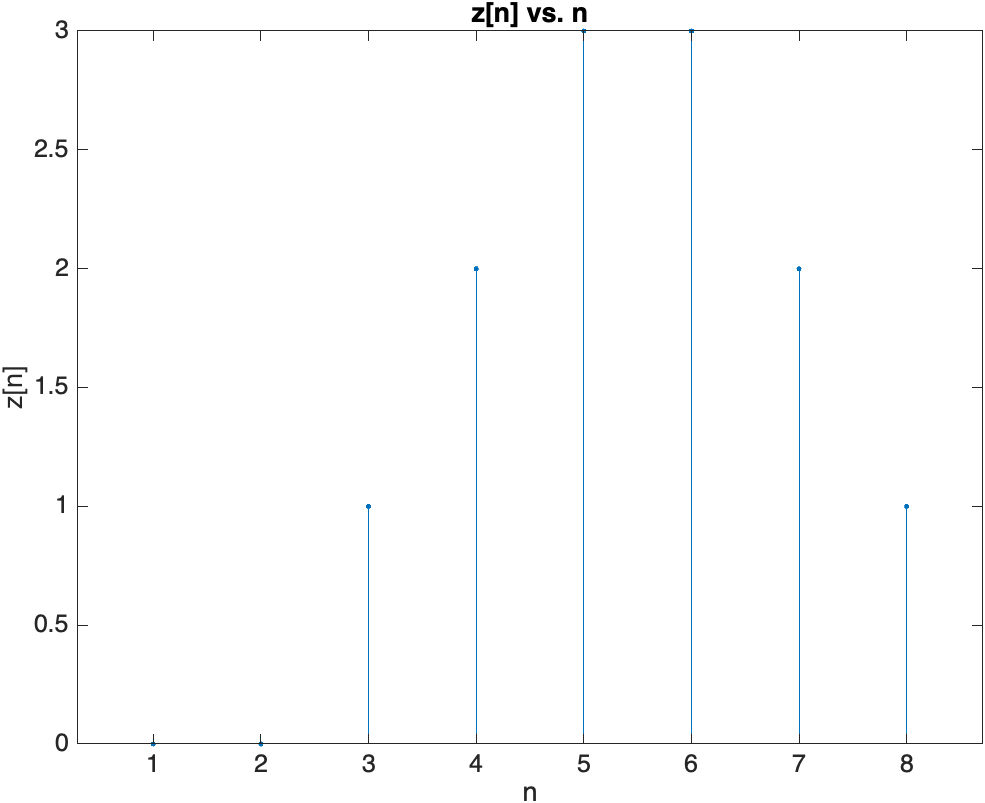
\includegraphics[width=0.5\linewidth]{ifft1.png}
\end{figure}
\begin{minted}[frame=single, fontsize=\small, linenos, bgcolor=white]{matlab}
a_k = fft(x_arr);
b_k = fft(y_arr);
c_k = a_k .* b_k;
z_arr = ifft(c_k);

stem(1:N, z_arr, '.');
title('z[n] vs. n', 'FontSize', 16);
xlabel('n', 'FontSize', 16);
ylabel('z[n]', 'FontSize', 16);
\end{minted}
We can then conclude it is similar to the one we obtained in \textbf{(e)}, its only difference being the time shift. We can directly compare values to analyze this, and we can observe
\begin{equation}
    z[n]=c[n-1].
\end{equation}

\item Comparing this to a linear convolution, which assumes the signal is aperiodic, we can obtain the following plot:
\begin{figure} [H]
    \centering
    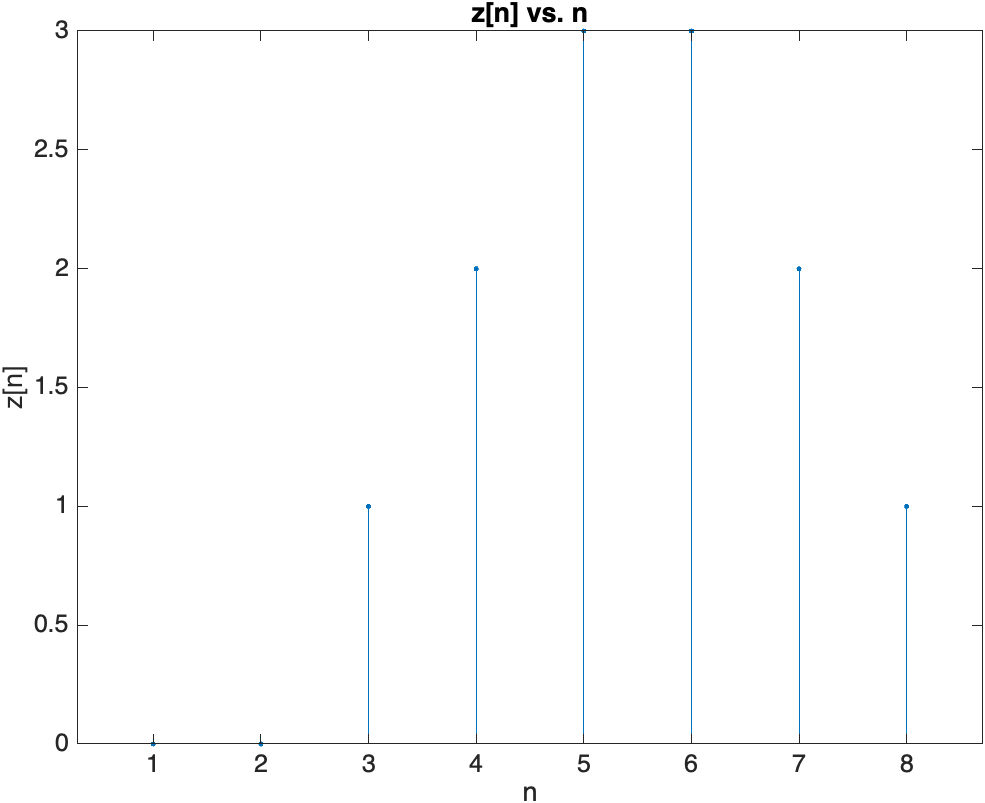
\includegraphics[width=0.5\linewidth]{conv2.png}
\end{figure}
\begin{minted}[frame=single, fontsize=\small, linenos, bgcolor=white]{matlab}
z_conv_linear = conv(x_arr, y_arr);
z_conv_linear = z_conv_linear(1:N)

stem(1:N, z_conv_linear, '.');
title('z[n] vs. n', 'FontSize', 16);
xlabel('n', 'FontSize', 16);
ylabel('z[n]', 'FontSize', 16);
\end{minted}
This plot is exactly the same as the one obtained in \textbf{(f)} and \textbf{(g)}, where it is
\begin{equation}
    z[n]=c[n-1]
\end{equation}
in relation to the one obtained in \textbf{(e)}.

\item Repeating parts \textbf{(a)} through \textbf{(h)} with the new signal, we can analyze the plots pictured below, and we can observe a similar relationship between each convolution method. However, one significant difference for the linear convolution result is the loss of data in this method. At the beginning of the signal, we have zeros where the other plots have non-zero values, which was not as apparent in the initial attempts as our values there were meant to be zeros. With this new $x[n]$, however, they are not meant to be zeros. We can verify this as both other methods give non-zero values for $n=1$ and $n=2$. They are still equivalent results for all other values, however.
\begin{figure} [H]
    \centering
    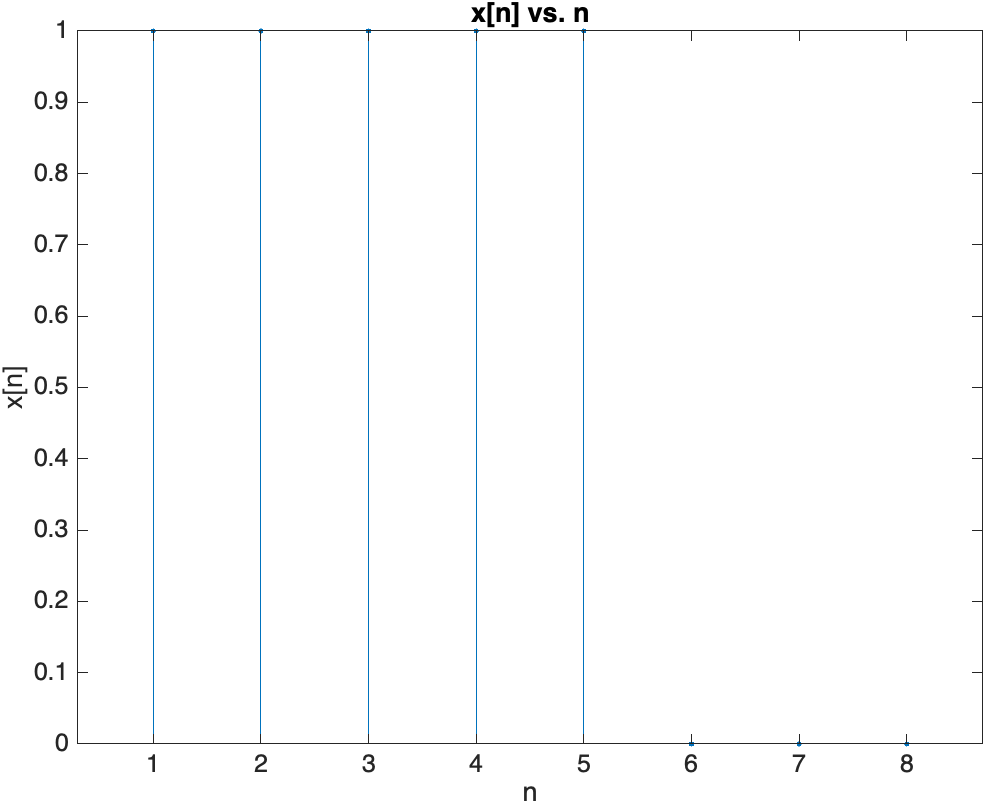
\includegraphics[width=0.32\linewidth]{20.png} 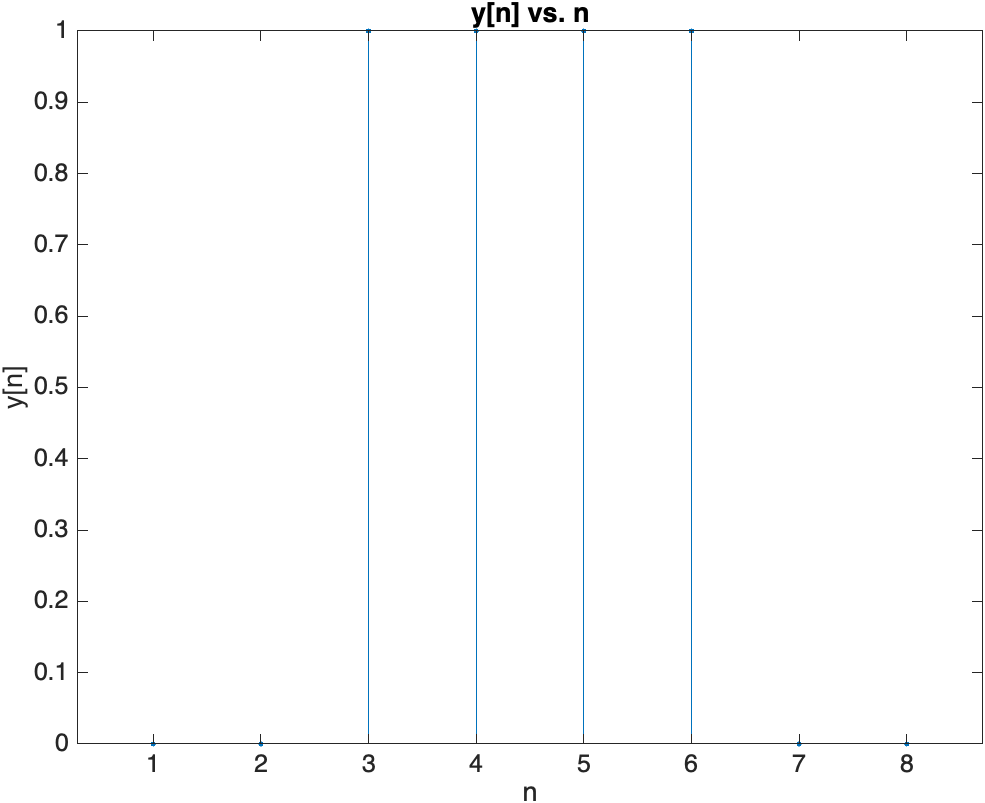
\includegraphics[width=0.32\linewidth]{21.png}    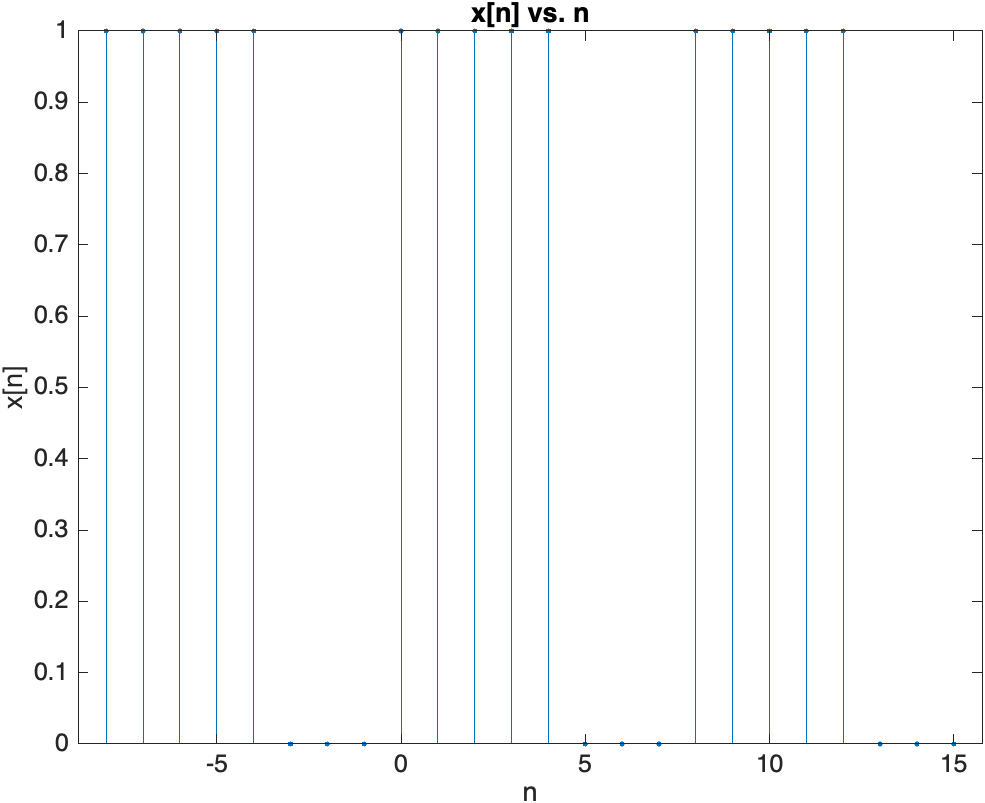
\includegraphics[width=0.32\linewidth]{22.png} 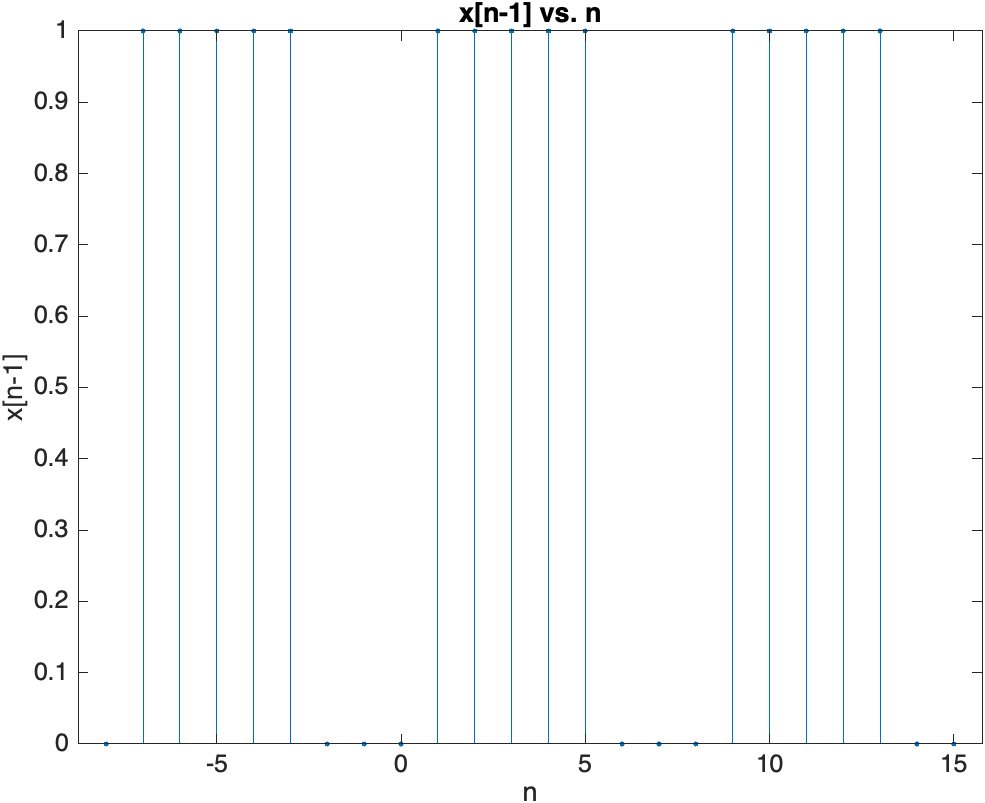
\includegraphics[width=0.32\linewidth]{23.png} 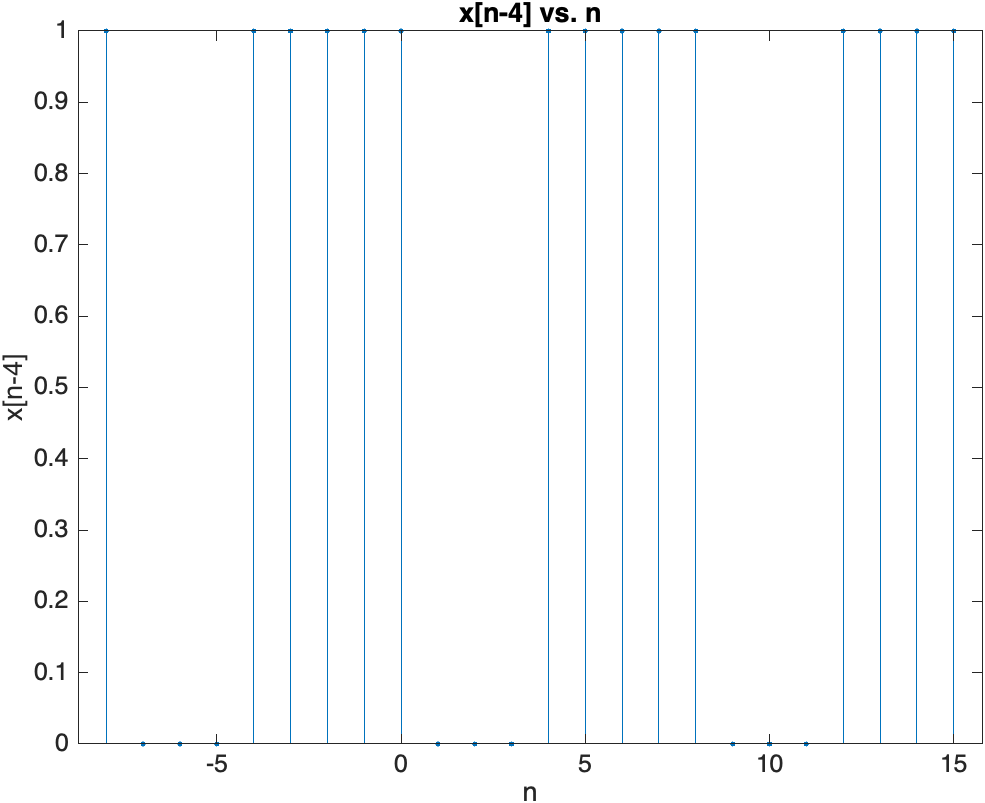
\includegraphics[width=0.32\linewidth]{24.png} 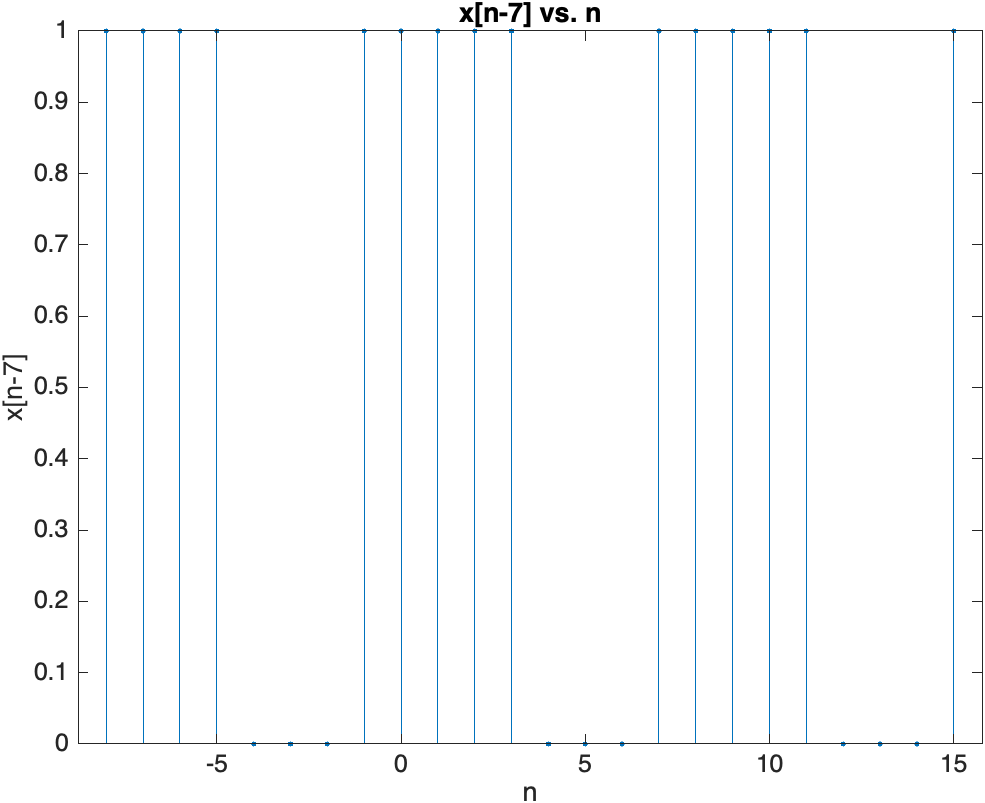
\includegraphics[width=0.32\linewidth]{25.png} 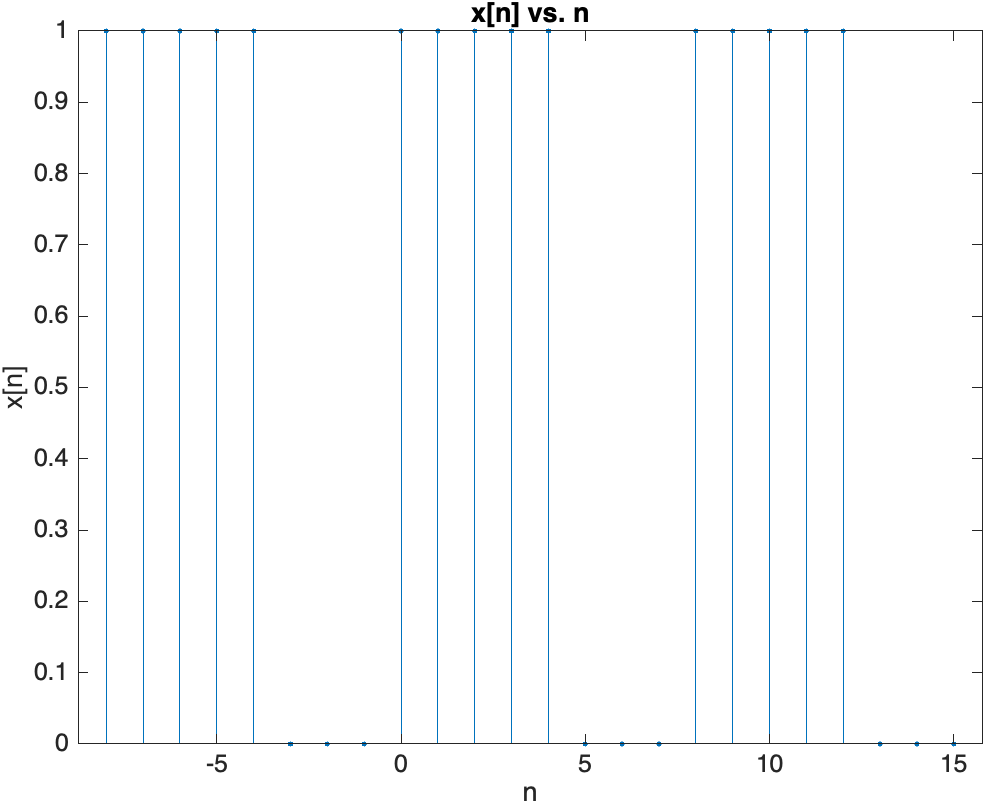
\includegraphics[width=0.32\linewidth]{26.png}    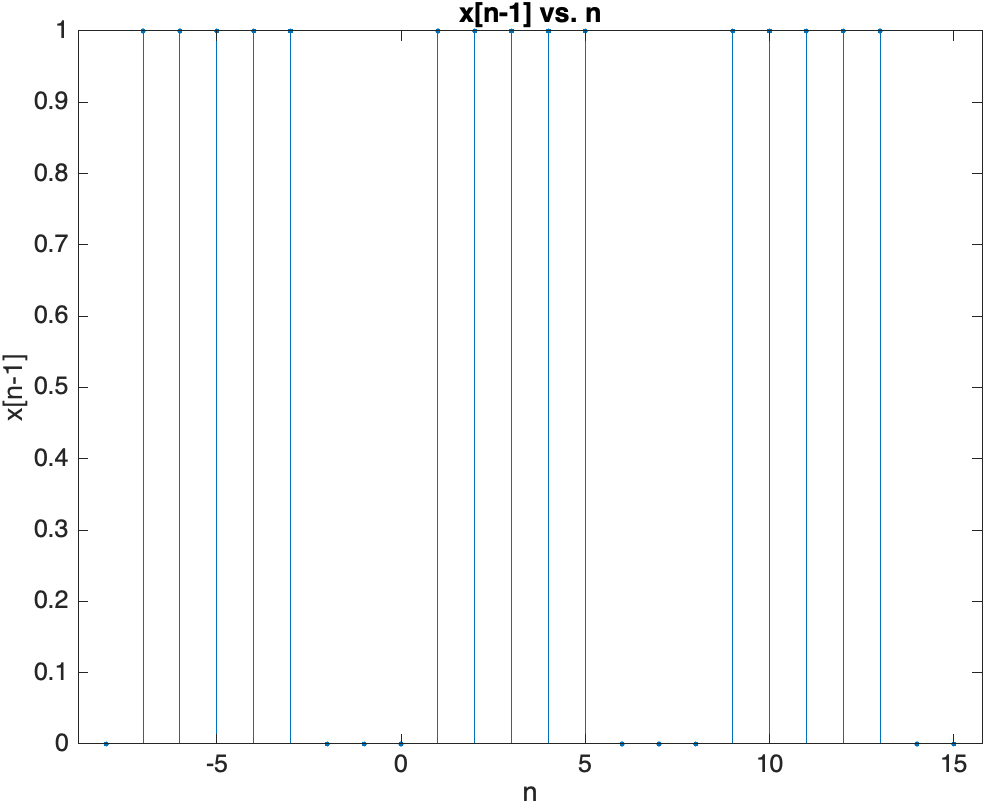
\includegraphics[width=0.32\linewidth]{27.png} 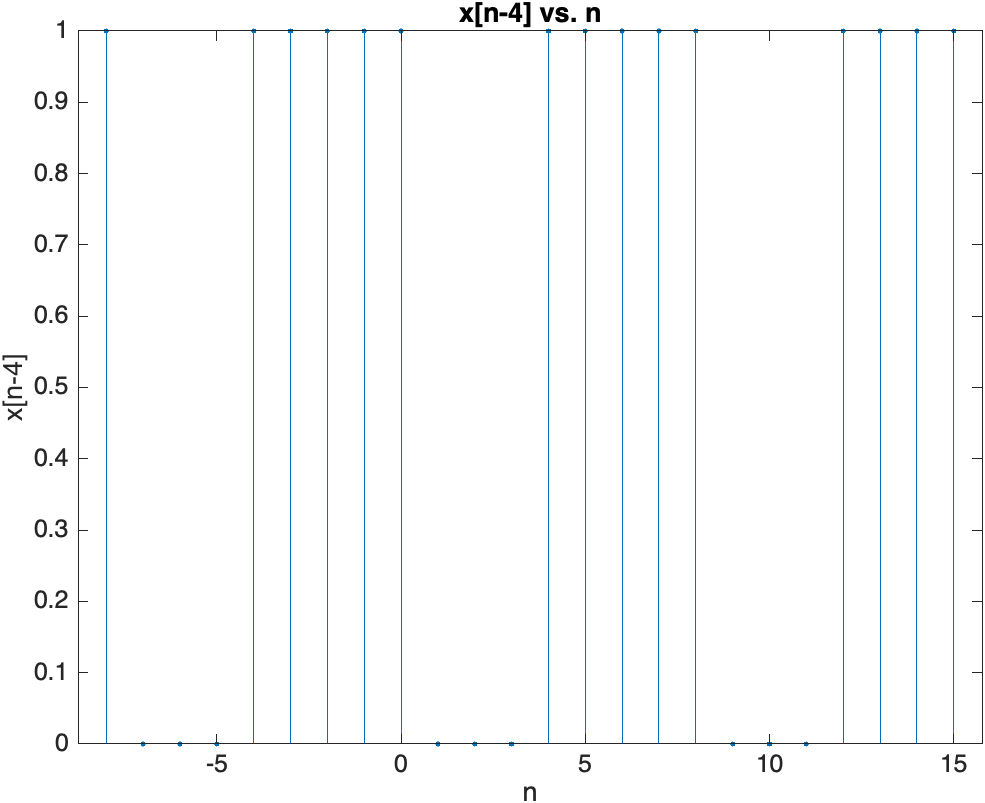
\includegraphics[width=0.32\linewidth]{28.png} 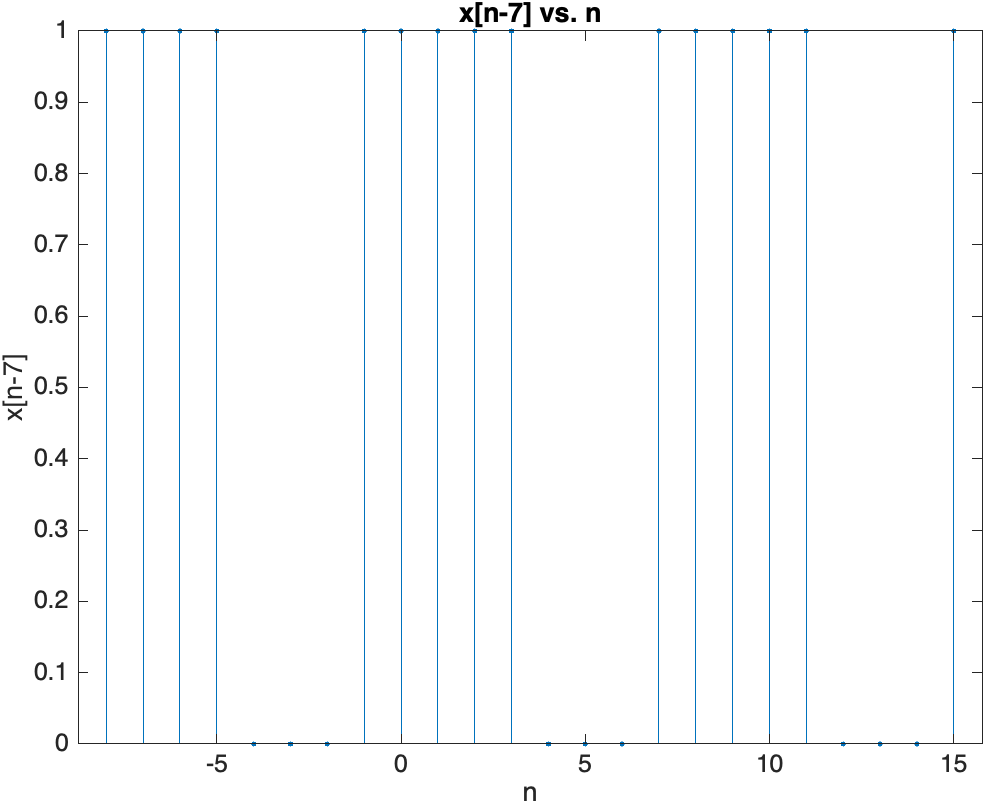
\includegraphics[width=0.32\linewidth]{29.png} 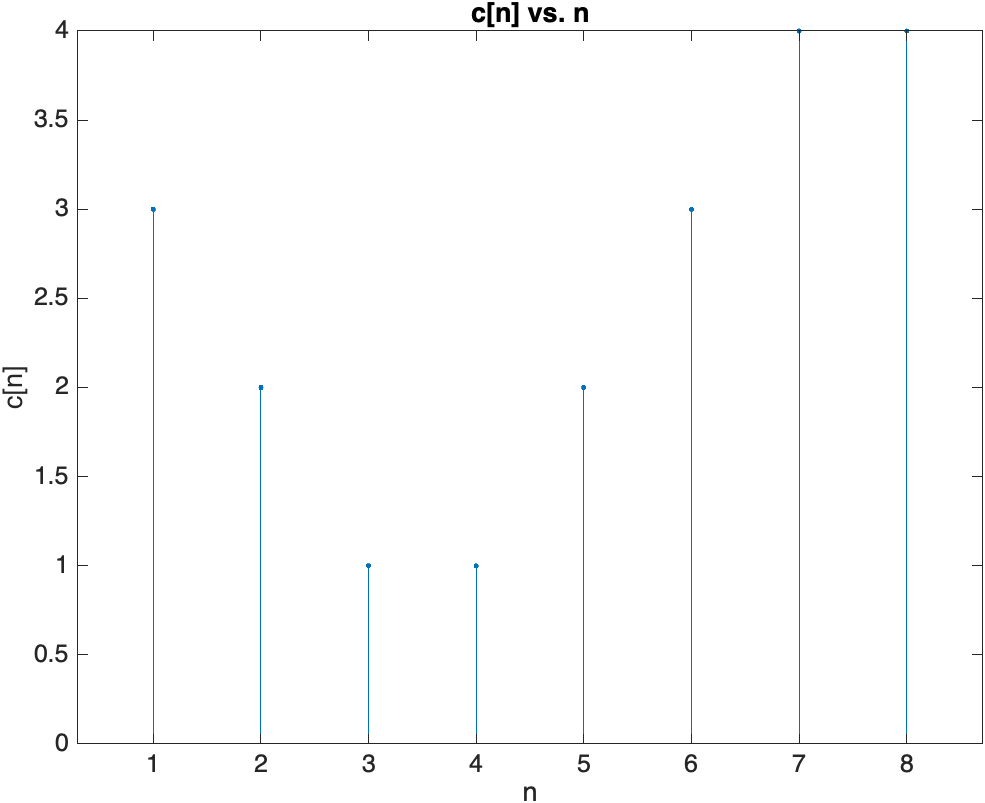
\includegraphics[width=0.32\linewidth]{30.png} 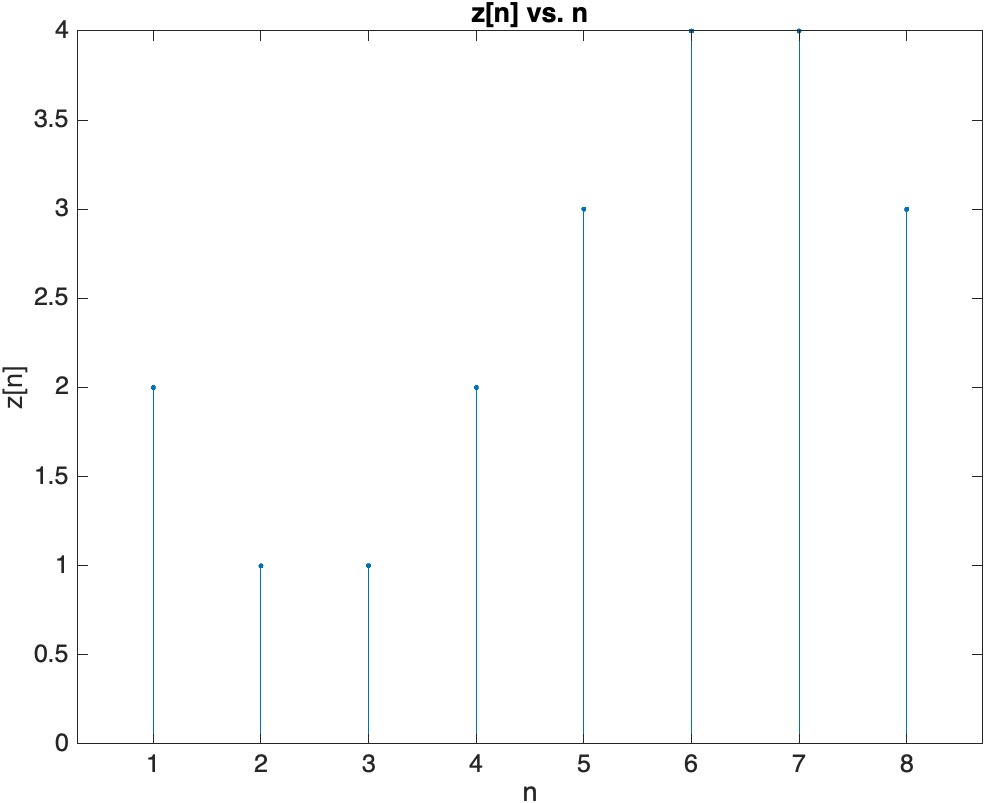
\includegraphics[width=0.32\linewidth]{31.png}    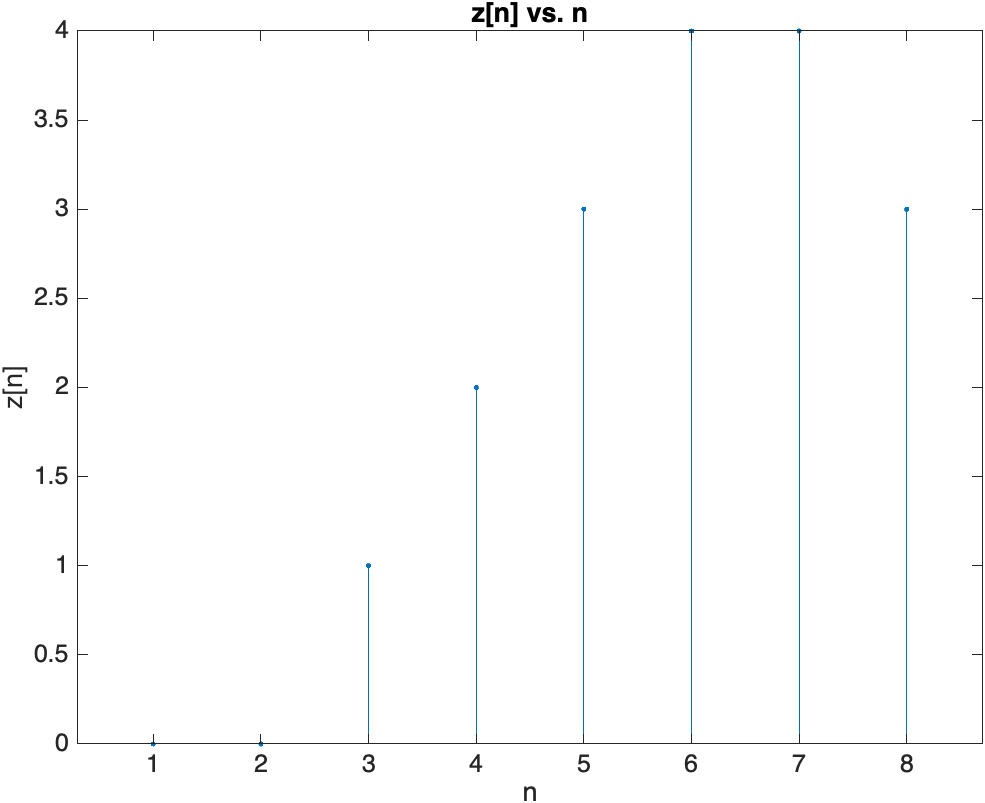
\includegraphics[width=0.5\linewidth]{32.png}
\end{figure}
\begin{minted}[frame=single, fontsize=\small, linenos, bgcolor=white]{matlab}
clear
n = 1:8;
x_arr = zeros(1,8);
y_arr = zeros(1,8);
x_arr(1:5) = 1;
y_arr(3:6) = 1;

stem(n, x_arr, '.');
title('x[n] vs. n', 'FontSize', 16);
xlabel('n', 'FontSize', 16);
ylabel('x[n]', 'FontSize', 16);

stem(n, y_arr, '.');
title('y[n] vs. n', 'FontSize', 16);
xlabel('n', 'FontSize', 16);
ylabel('y[n]', 'FontSize', 16);

n = -8:15;
x_arr3 = zeros(1, length(n));
for i = 0:2
    x_arr3(8*i+1:8*(i+1))=x_arr;
end

stem(n, x_arr3, '.');
title('x[n] vs. n', 'FontSize', 16)
xlabel('n', 'FontSize', 16);
ylabel('x[n]', 'FontSize', 16);

x_ext=x_arr3;
x_ext(25:48)=x_arr3;

shiftval=1;
stem(n, x_ext(9-shiftval:32-shiftval), '.');
title('x[n-1] vs. n', 'FontSize', 16);
xlabel('n', 'FontSize', 16);
ylabel('x[n-1]', 'FontSize', 16);

shiftval=4;
stem(n, x_ext(9-shiftval:32-shiftval), '.');
title('x[n-4] vs. n', 'FontSize', 16);
xlabel('n', 'FontSize', 16);
ylabel('x[n-4]', 'FontSize', 16);

shiftval=7;
stem(n, x_ext(9-shiftval:32-shiftval), '.');
title('x[n-7] vs. n', 'FontSize', 16);
xlabel('n', 'FontSize', 16);
ylabel('x[n-7]', 'FontSize', 16);

stem(n, circshift(x_arr3, 0), '.');
title('x[n] vs. n', 'FontSize', 16);
xlabel('n', 'FontSize', 16);
ylabel('x[n]', 'FontSize', 16);

stem(n, circshift(x_arr3, 1), '.');
title('x[n-1] vs. n', 'FontSize', 16);
xlabel('n', 'FontSize', 16);
ylabel('x[n-1]', 'FontSize', 16);

stem(n, circshift(x_arr3, 4), '.');
title('x[n-4] vs. n', 'FontSize', 16);
xlabel('n', 'FontSize', 16);
ylabel('x[n-4]', 'FontSize', 16);

stem(n, circshift(x_arr3, 7), '.');
title('x[n-7] vs. n', 'FontSize', 16);
xlabel('n', 'FontSize', 16);
ylabel('x[n-7]', 'FontSize', 16);

N = 8;
c_arr = zeros(1, N);
% Remember that convolution has to happen over any one period. 
% 1:N is convenient
for idx = 1:N
    % First flip
    y_flipped = y_arr(N:-1:1);

    % Then advance using circshift
    y_shifted = circshift(y_flipped, idx-1);
    c_arr(idx) = sum(x_arr.*y_shifted);
end

stem(1:N, c_arr, '.')
title('c[n] vs. n', 'FontSize', 16);
xlabel('n', 'FontSize', 16);
ylabel('c[n]', 'FontSize', 16);

a_k = fft(x_arr);
b_k = fft(y_arr);
c_k = a_k .* b_k;
z_arr = ifft(c_k);

stem(1:N, z_arr, '.');
title('z[n] vs. n', 'FontSize', 16);
xlabel('n', 'FontSize', 16);
ylabel('z[n]', 'FontSize', 16);

z_conv_linear = conv(x_arr, y_arr);
z_conv_linear = z_conv_linear(1:N);

stem(1:N, z_conv_linear, '.');
title('z[n] vs. n', 'FontSize', 16);
xlabel('n', 'FontSize', 16);
ylabel('z[n]', 'FontSize', 16);
\end{minted}

\end{enumerate}
\end{document}